\subsection{Mô hình nhận diện ký hiệu ở tầng thị giác}

Mô-đun đầu tiên của hệ thống chịu trách nhiệm biến dữ liệu video thành một chuỗi gloss trung gian để
đưa sang tầng xử lý ngôn ngữ. Về mặt chức năng, đây là khối ``đọc'' cử chỉ của người dùng thông qua
webcam. Về mặt kỹ thuật, hệ thống sử dụng MediaPipe Holistic để trích xuất toàn bộ landmarks cơ thể
từ mỗi frame video, sau đó đưa chuỗi landmarks theo thời gian vào một mô hình TFLite pre-trained
(giải pháp đạt giải nhất cuộc thi Kaggle ASL Signs) để dự đoán nhãn ký hiệu.

Cần nhấn mạnh một điểm quan trọng để báo cáo trung thực với hiện trạng dự án: mô-đun này sử dụng
mô hình đã được huấn luyện sẵn trên bộ dữ liệu Kaggle ASL Signs gồm 250 từ vựng ký hiệu ASL. Mô
hình không được nhóm tự huấn luyện từ đầu, mà được tích hợp như một thành phần pre-trained trong
pipeline nhận diện. Sau khi dự đoán nhãn tiếng Anh, hệ thống ánh xạ sang gloss trung gian tiếng Việt
để nối với mô-đun NLP phía sau.

\begin{figure}[H]
\centering
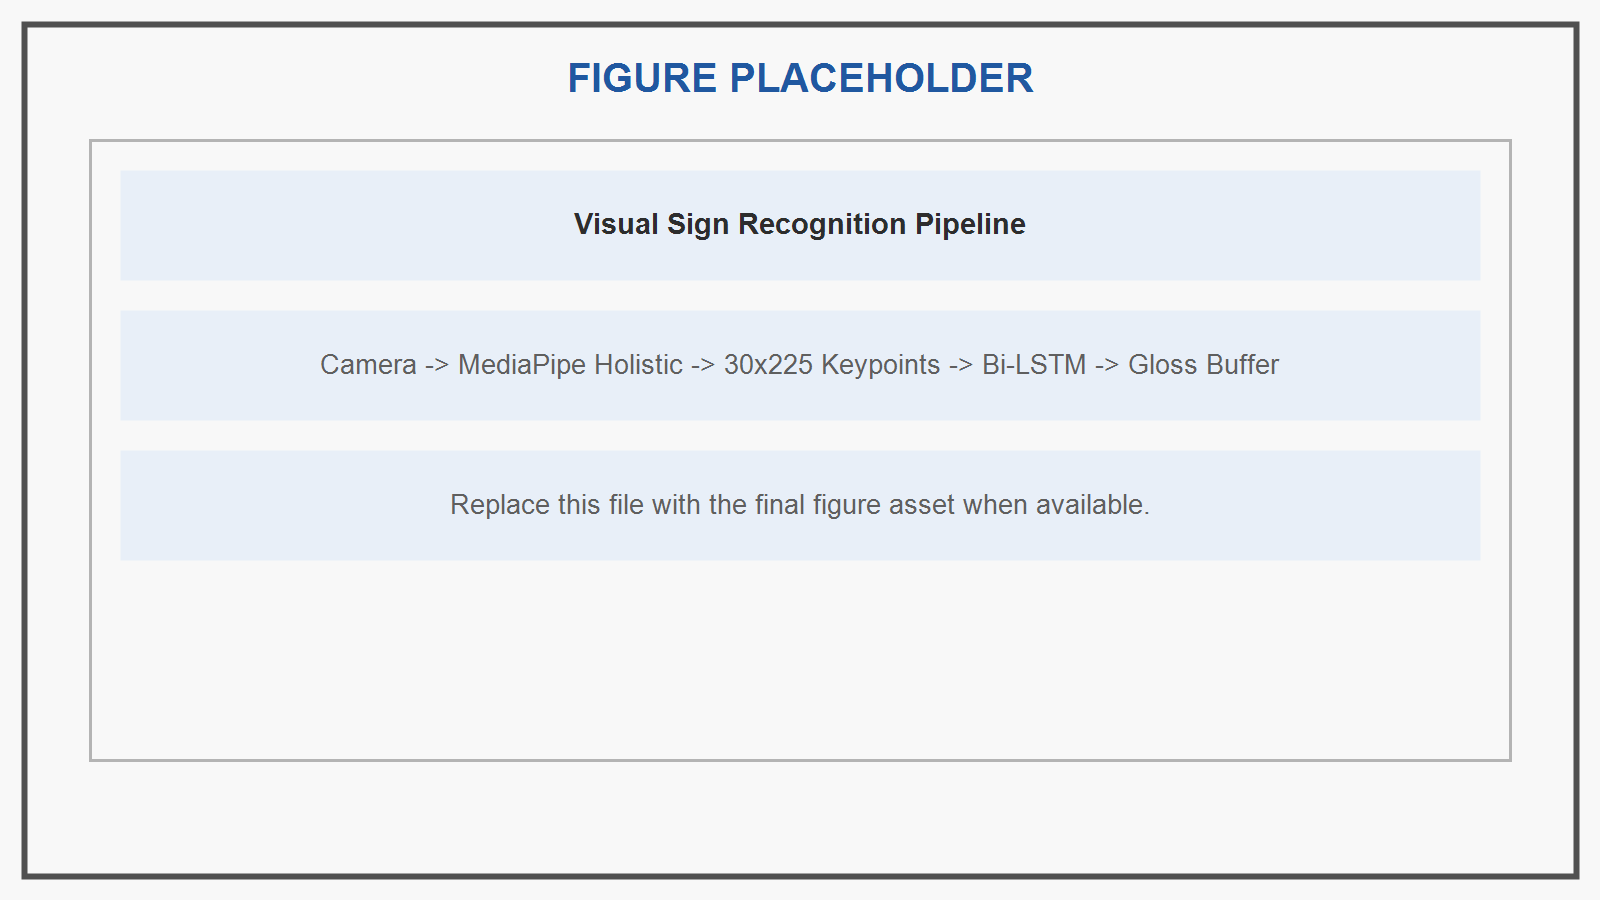
\includegraphics[width=0.88\textwidth]{figures/recognition/vsl_recognition_pipeline.png}
\caption{Vị trí của mô-đun nhận diện thị giác trong pipeline tổng thể}
\label{fig:vsl-recognition-pipeline}
\end{figure}

\subsubsection{Phát biểu bài toán}

Xét một đoạn video ngắn hoặc một cửa sổ trượt gồm nhiều frame liên tiếp từ webcam, mục tiêu của mô
hình là dự đoán ra một nhãn từ vựng ký hiệu tương ứng. Trong dự án này, đầu ra của mô hình là một
\textit{gloss} ở mức từ hoặc cụm từ ngắn, ví dụ \texttt{drink}, \texttt{hello}, \texttt{help},
\texttt{food}. Gloss đó sau đó có thể được ánh xạ sang token tiếng Việt tương ứng.

Do ký hiệu là tín hiệu có tính động, bài toán không thể chỉ nhìn một frame đơn lẻ. Ý nghĩa của một
từ ký hiệu thường phụ thuộc đồng thời vào:
\begin{itemize}
    \item vị trí tương đối giữa tay, vai, khuỷu tay và thân người;
    \item hình dạng và quỹ đạo chuyển động của hai bàn tay;
    \item biểu cảm khuôn mặt và hướng nhìn;
    \item thứ tự diễn tiến của các động tác theo thời gian.
\end{itemize}

Vì vậy, mô hình được thiết kế như một bộ phân loại đa lớp trên \textit{chuỗi đặc trưng theo thời
gian}, thay vì trên từng ảnh tĩnh.

\subsubsection{Vai trò của MediaPipe Holistic trong pipeline}

Theo tài liệu chính thức của Google, MediaPipe Holistic có thể xuất tổng cộng 543 landmarks trong
thời gian thực, bao gồm 468 điểm khuôn mặt, 33 điểm pose và 21 điểm cho mỗi bàn tay. Khác với
phiên bản trước của dự án (chỉ dùng pose và bàn tay với 225 đặc trưng), mô hình hiện tại giữ lại
\textbf{toàn bộ 543 landmarks} để tận dụng tối đa thông tin về biểu cảm khuôn mặt, thân trên và
hai bàn tay. Đây là lựa chọn phù hợp vì:
\begin{itemize}
    \item mô hình TFLite đã được huấn luyện trên toàn bộ 543 landmarks, nên đầu vào phải giữ nguyên
    cấu trúc này;
    \item landmarks khuôn mặt bổ sung thêm tín hiệu biểu cảm quan trọng cho nhiều từ ký hiệu;
    \item MediaPipe Holistic đã được tối ưu cho luồng ảnh liên tục, phù hợp với bài toán realtime
    trên webcam.
\end{itemize}

\begin{figure}[H]
\centering
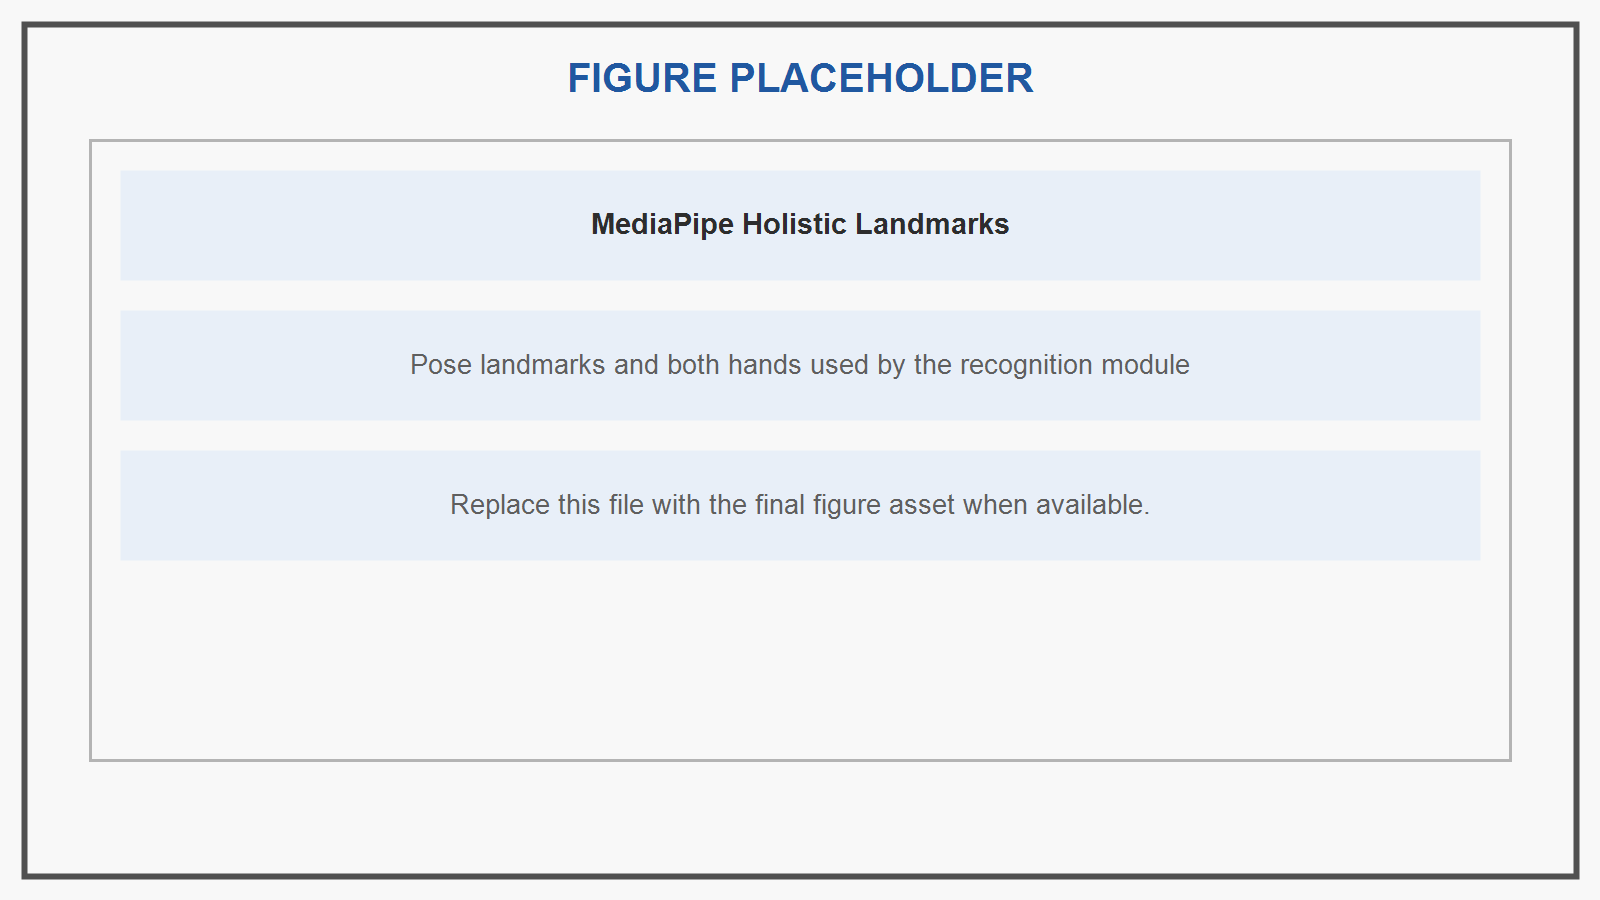
\includegraphics[width=0.84\textwidth]{figures/recognition/mediapipe_holistic_landmarks.png}
\caption{Minh họa landmarks pose, khuôn mặt và bàn tay được trích xuất bởi MediaPipe Holistic}
\label{fig:mediapipe-holistic-landmarks}
\end{figure}

\begin{table}[H]
\centering
\caption{Thành phần vector đặc trưng ở mỗi frame}
\label{tab:recognition-feature-layout}
\begin{tabularx}{\textwidth}{|p{3.4cm}|c|c|c|}
\hline
\textbf{Thành phần} & \textbf{Số điểm} & \textbf{Số tọa độ/điểm} & \textbf{Tổng đặc trưng} \\
\hline
Khuôn mặt & 468 & 3 & 1.404 \\
\hline
Tay trái & 21 & 3 & 63 \\
\hline
Pose & 33 & 3 & 99 \\
\hline
Tay phải & 21 & 3 & 63 \\
\hline
\textbf{Tổng} & \textbf{543} & \textbf{3} & \textbf{1.629} \\
\hline
\end{tabularx}
\end{table}

\subsubsection{Biểu diễn đầu vào theo chuỗi landmarks}

Sau khi một frame được biến thành ma trận landmarks kích thước \texttt{543 x 3}, hệ thống gom
các frame liên tiếp thành một chuỗi có độ dài linh hoạt. Trong code hiện tại
(\texttt{realtime\_asl\_250.py}), cửa sổ trượt có kích thước tối đa 60 frame và yêu cầu tối thiểu
16 frame trước khi bắt đầu suy luận. Kết quả là mỗi lần suy luận nhận đầu vào là một tensor
kích thước \texttt{N x 543 x 3}, với \texttt{N} nằm trong khoảng \texttt{[16, 60]}.

Điểm khác biệt quan trọng so với các thiết kế chuỗi cố định là mô hình TFLite có khả năng nhận
đầu vào có chiều dài thay đổi nhờ cơ chế \texttt{resize\_tensor\_input()}. Điều này mang lại hai
lợi ích:
\begin{itemize}
    \item mô hình có thể bắt đầu dự đoán sớm ngay khi có đủ 16 frame, giảm độ trễ ban đầu;
    \item khi cửa sổ trượt đầy (60 frame), mô hình có nhiều ngữ cảnh hơn để phân loại chính xác.
\end{itemize}

Một chi tiết kỹ thuật quan trọng trong code là nếu frame bị mất landmark, hệ thống sẽ đệm bằng
\texttt{NaN} thay vì vector zero. Đây là quy ước của mô hình Kaggle ASL Signs: giá trị \texttt{NaN}
cho phép mô hình phân biệt giữa ``không có tay'' và ``tay ở vị trí gốc tọa độ''.

\begin{figure}[H]
\centering
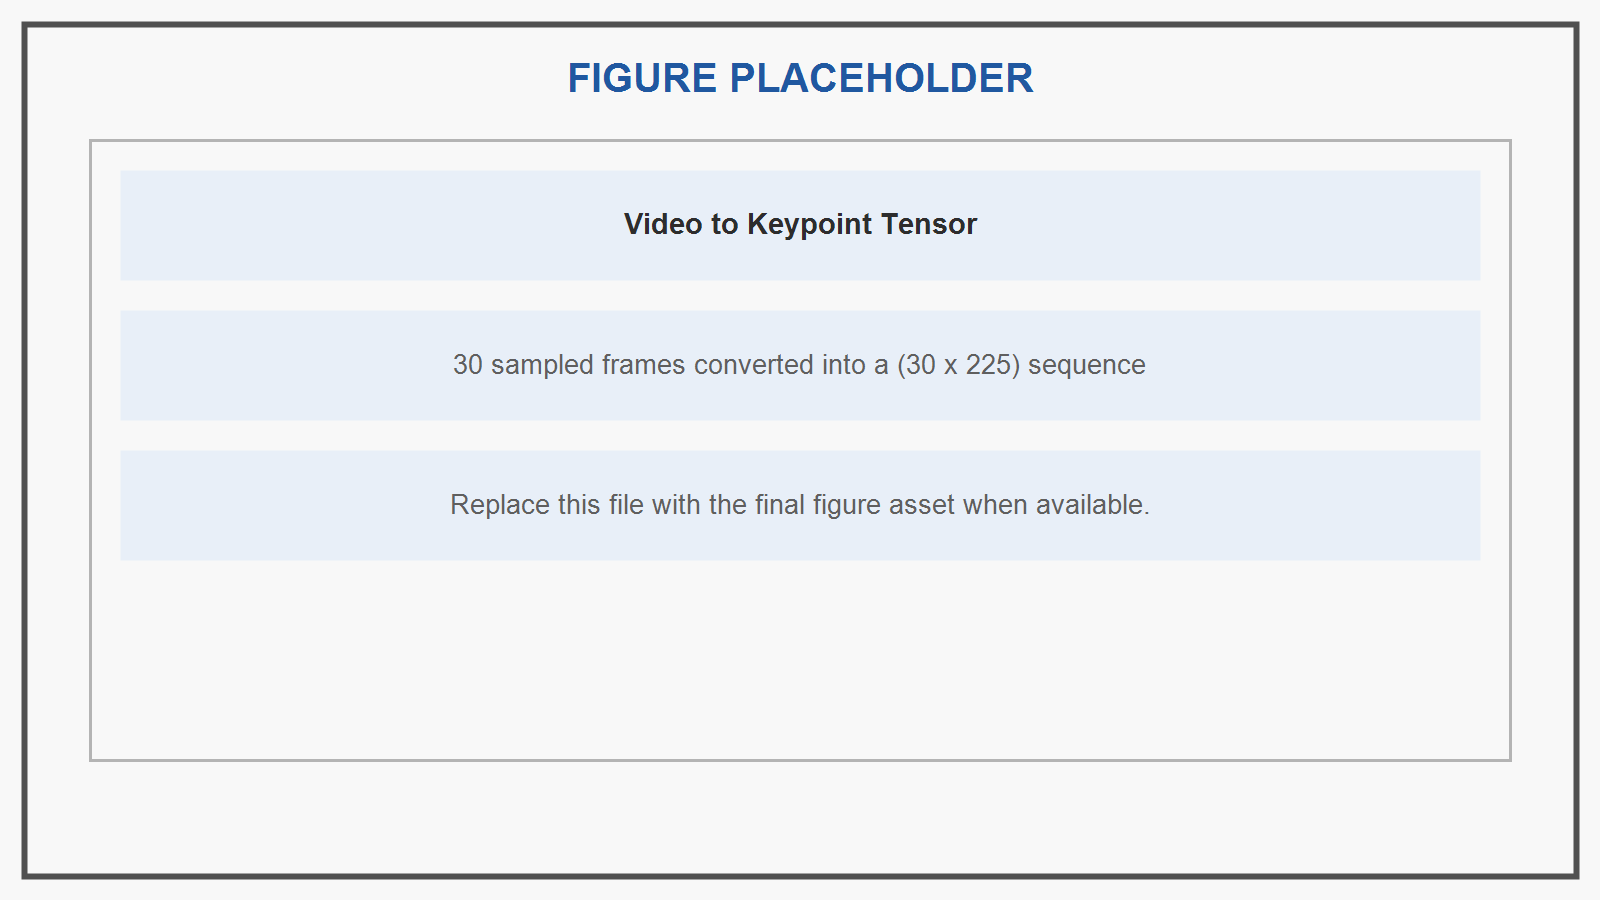
\includegraphics[width=0.82\textwidth]{figures/recognition/keypoint_vectorization.png}
\caption{Sơ đồ biến video thành chuỗi landmarks kích thước N x 543 x 3}
\label{fig:keypoint-vectorization}
\end{figure}

\subsubsection{Kiến trúc mô hình TFLite (Kaggle ASL Signs 1st Place)}

Mô hình nhận diện trong dự án là giải pháp đạt giải nhất cuộc thi
\textit{Google -- Isolated Sign Language Recognition} trên Kaggle. Mô hình đã được chuyển đổi
sang định dạng TensorFlow Lite (\texttt{model.tflite}) để tối ưu cho suy luận nhanh trên thiết
bị đầu cuối.

Về kiến trúc, mô hình này khác biệt hoàn toàn so với các mạng hồi quy truyền thống:
\begin{itemize}
    \item đầu vào là chuỗi landmarks có chiều dài linh hoạt, mỗi frame gồm 543 điểm x 3 tọa độ;
    \item mô hình được huấn luyện end-to-end trên dữ liệu landmarks, không cần bước trích xuất
    đặc trưng thủ công;
    \item đầu ra là phân bố xác suất trên 250 lớp từ vựng ký hiệu ASL;
    \item mô hình sử dụng TFLite Interpreter cho suy luận, cho phép chạy trên CPU mà không cần GPU.
\end{itemize}

Trong code, quá trình suy luận được thực hiện qua các bước:
\begin{enumerate}
    \item gom landmarks thành tensor đầu vào;
    \item gọi \texttt{interpreter.resize\_tensor\_input()} để điều chỉnh kích thước đầu vào
    theo số frame thực tế;
    \item gọi \texttt{interpreter.allocate\_tensors()} và \texttt{set\_tensor()};
    \item gọi \texttt{interpreter.invoke()} để chạy suy luận;
    \item lấy kết quả từ \texttt{get\_tensor()}, áp dụng softmax nếu cần;
    \item chọn top-k lớp có xác suất cao nhất.
\end{enumerate}

File \texttt{sign\_to\_prediction\_index\_map.json} chứa bảng ánh xạ giữa tên từ vựng ký hiệu
và chỉ số đầu ra của mô hình, cho phép chuyển đổi kết quả số thành nhãn có nghĩa.

\begin{table}[H]
\centering
\caption{Thông số chính của mô hình nhận diện}
\label{tab:recognition-hyperparameters}
\begin{tabularx}{\textwidth}{|p{5cm}|X|}
\hline
\textbf{Tham số} & \textbf{Giá trị trong code} \\
\hline
Số lớp từ vựng & 250 \\
\hline
Kích thước đầu vào mỗi frame & 543 landmarks x 3 tọa độ \\
\hline
Số frame tối thiểu & 16 \\
\hline
Số frame tối đa (sliding window) & 60 \\
\hline
Tần suất suy luận & Mỗi 8 frame \\
\hline
Top-k hiển thị & 3 \\
\hline
Định dạng mô hình & TensorFlow Lite (.tflite) \\
\hline
Kích thước file mô hình & $\sim$11 MB \\
\hline
\end{tabularx}
\end{table}

\subsubsection{Nguồn gốc mô hình và dữ liệu huấn luyện}

Mô hình TFLite được lấy từ giải pháp đạt giải nhất cuộc thi Kaggle
\textit{Google -- Isolated Sign Language Recognition}. Cuộc thi này yêu cầu các đội thi xây
dựng mô hình nhận diện 250 từ vựng ký hiệu ASL từ dữ liệu landmarks đã được trích xuất
bằng MediaPipe Holistic.

Dữ liệu huấn luyện gốc của cuộc thi bao gồm:
\begin{itemize}
    \item 250 từ vựng ký hiệu ASL phổ biến;
    \item dữ liệu landmarks đã được trích xuất sẵn (không phải video RGB);
    \item nhiều signer với điều kiện ghi hình khác nhau.
\end{itemize}

Vì đây là mô hình pre-trained, nhóm không thực hiện quá trình huấn luyện lại. Thay vào đó,
mô hình được sử dụng trực tiếp làm thành phần nhận diện trong pipeline tổng thể. Đây là một
lựa chọn thực dụng cho đồ án vì cho phép tập trung nguồn lực vào các tầng NLP phía sau,
đồng thời vẫn đảm bảo chất lượng nhận diện ở mức cạnh tranh nhờ vào kết quả đã được kiểm
chứng qua cuộc thi.

\subsubsection{Cơ chế suy luận thời gian thực}

Trong \texttt{realtime\_asl\_250.py}, hệ thống duy trì một bộ đệm trượt:
\begin{itemize}
    \item \texttt{frames = deque(maxlen=60)};
    \item chỉ gom frame khi phát hiện có bàn tay (trái hoặc phải) xuất hiện trong khung hình;
    \item suy luận mỗi 8 frame (\texttt{predict\_every=8});
    \item chỉ bắt đầu suy luận khi bộ đệm đủ tối thiểu 16 frame;
    \item hiển thị top-3 dự đoán có xác suất cao nhất;
    \item nhấn phím Space để reset bộ đệm, phím \texttt{q} để thoát.
\end{itemize}

Thiết kế ``chỉ gom khi có tay'' là một cải tiến quan trọng: thay vì gom mọi frame kể cả khi
người dùng không ký hiệu, hệ thống chỉ thu thập dữ liệu khi phát hiện ít nhất một bàn tay.
Điều này giúp giảm nhiễu đầu vào và tăng chất lượng dự đoán.

\subsubsection{Ưu điểm và giới hạn của thiết kế hiện tại}

Thiết kế \textit{MediaPipe Holistic + TFLite pre-trained} có một số ưu điểm rõ ràng:
\begin{itemize}
    \item mô hình đã được kiểm chứng qua cuộc thi Kaggle với chất lượng cao;
    \item sử dụng toàn bộ 543 landmarks bao gồm cả biểu cảm khuôn mặt;
    \item kiến trúc gọn, suy luận bằng TFLite trên CPU, phù hợp với phần cứng phổ thông;
    \item cửa sổ trượt linh hoạt 16--60 frame và logic ``chỉ gom khi có tay'' phù hợp cho
    demo realtime;
    \item đầu ra gloss là giao diện trung gian thuận lợi để nối với tầng NLP.
\end{itemize}

Mặt khác, vẫn còn các giới hạn quan trọng:
\begin{itemize}
    \item mô hình được huấn luyện trên dữ liệu ASL, không phải VSL gốc, nên tính đúng đắn
    ngôn ngữ còn phụ thuộc bước ánh xạ gloss;
    \item số lớp từ vựng là 250, ít hơn so với nhu cầu giao tiếp thực tế;
    \item mô hình hiện nhận diện ở mức từ đơn lẻ, chưa xử lý trực tiếp câu ký hiệu liên tục;
    \item vì là mô hình pre-trained, nhóm không thể can thiệp vào kiến trúc bên trong hoặc
    tinh chỉnh cho VSL;
    \item chất lượng cuối cùng của pipeline chịu ảnh hưởng mạnh từ ánh sáng, góc quay, che khuất
    tay và sự khác biệt giữa signer thật với signer trong dữ liệu Kaggle.
\end{itemize}

